\subsection{UC2 – Area Personale}
\begin{center}
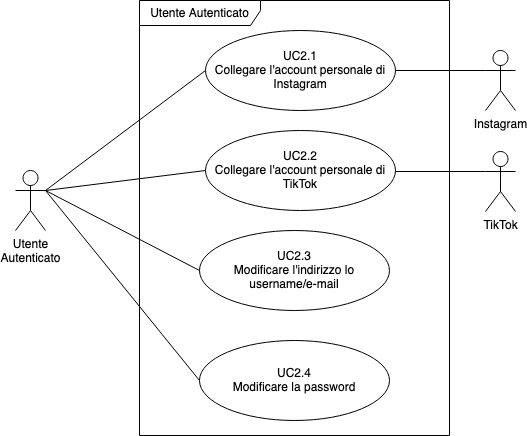
\includegraphics[scale=0.5]{UC_images/UC2.png}
\end{center}
\subsubsection{UC2.1 – Collegare l'Account Instagram}
\begin{center}
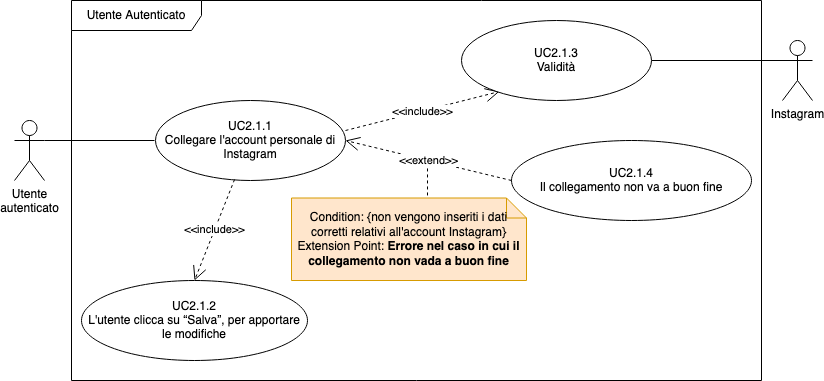
\includegraphics[scale=0.5]{UC_images/UC2_1.png}
\end{center}
\begin{itemize}
\item \textbf{Attore primario}: Utente autenticato
\item \textbf{Attore secondario}: Instagram
\item \textbf{Precondizione}: L’utente è autenticato nel sistema
\item \textbf{Postcondizione}: L’utente ha collegato il suo account Instagram al sistema

\item \textbf{Scenario principale}:
\begin{enumerate}
\item L’utente collega il suo account personale di Instagram
\item Per confermare l’azione, l’utente deve cliccare su “Salva” 
\end{enumerate}

\item \textbf{Estensioni}:
\begin{itemize}
\item Il collegamento all’account Instagram non va a buon fine
\begin{enumerate}
	\item L’utente prova a collegare il proprio account Instagram all’account registrato nel sistema, cliccando il bottone “Instagram”;
	\item L’accesso alla piattaforma Instagram non va a buon fine, poiché non vengono inseriti i dati di accesso corretti (UC2.1.4 §).
	%\item All’utente viene offerta la possibilità di effettuare un nuovo collegamento
\end{enumerate}
\end{itemize}

\item \textbf{Inclusioni}:
\begin{itemize}
\item Verifica validità link (UC3.2 §3.8).
\end{itemize}
\end{itemize}

\subsubsection{UC2.2 – Collegare l'Account TikTok}
\begin{center}
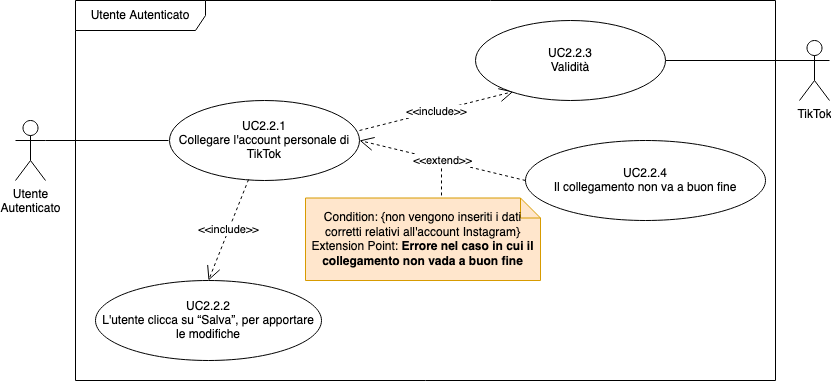
\includegraphics[scale=0.5]{UC_images/UC2_2.png}
\end{center}
\begin{itemize}
\item \textbf{Attore primario}: Utente autenticato.
\item \textbf{Attore secondario}: TikTok.
\item \textbf{Precondizione}: L’utente è autenticato nel sistema.
\item \textbf{Postcondizione}: L’utente ha collegato il suo account TikTok al sistema.

\item \textbf{Scenario principale}:
\begin{enumerate}
\item L’utente collega il suo account personale di TikTok;
\item Per confermare l’azione, l’utente deve cliccare su “Salva”. 
\end{enumerate}

\item \textbf{Estensioni}:
\begin{itemize}
\item Il collegamento all’account Instagram non va a buon fine
\begin{enumerate}
	\item L’utente prova a collegare il proprio account TikTok all’account registrato nel sistema, cliccando il bottone TikTok;
	\item L’accesso alla piattaforma TikTok non va a buon fine, poiché non vengono inseriti i dati di accesso corretti (UC2.2.4 §).
\end{enumerate}
\end{itemize}

\item \textbf{Inclusioni}:
\begin{itemize}
\item Verifica validità link (UC3.2 §3.8).
\end{itemize}
\end{itemize}

\subsubsection{UC2.3 – Modifica dell'indirizzo e-mail/username}
\begin{center}
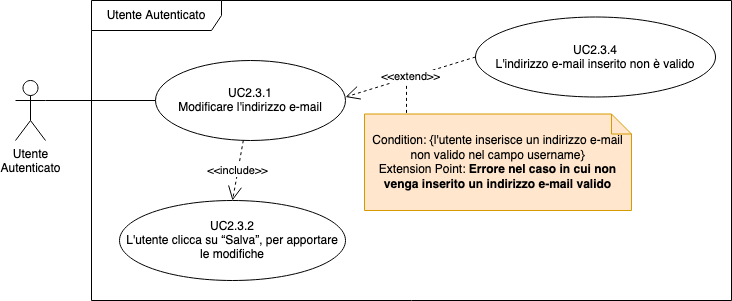
\includegraphics[scale=0.5]{UC_images/UC2_3.png}
\end{center}
\begin{itemize}
\item \textbf{Attore primario}: Utente autenticato.
\item \textbf{Precondizione}: L’utente è autenticato nel sistema.
\item \textbf{Postcondizione}: L’utente ha inserito un indirizzo e-mail valido ed ha modificato il campo e-mail/username.

\item \textbf{Scenario principale}:
\begin{enumerate}
\item L’utente inserisce il nuovo indirizzo e-mail nel campo e-mail/username;
\item L’utente clicca su “Salva” per aggiornare l'indirizzo e-mail registrato nella piattaforma.
\end{enumerate}

\item \textbf{Estensioni}:
\begin{itemize}
\item L’utente inserisce un indirizzo e-mail non valido
\begin{enumerate}
	\item L’utente inserisce un nuovo indirizzo e-mail nel campo e-mail/username;
	\item Il sistema rileva che l’indirizzo inserito non è valido (UC2.3.4 §).
	%\item Il sistema non modifica l’indirizzo e-mail e mantiene il vecchio indirizzo;
	%\item All’utente viene data la possibilità di modificare lo username inserendo nuovamente un indirizzo e-mail valido.
\end{enumerate}
\end{itemize}
\end{itemize}

\subsubsection{UC2.4 – Modifica della password}
\begin{center}
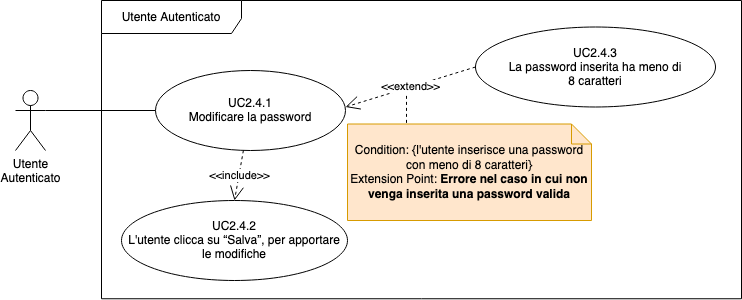
\includegraphics[scale=0.5]{UC_images/UC2_4.png}
\end{center}
\begin{itemize}
\item \textbf{Attore primario}: Utente autenticato
\item \textbf{Precondizione}: L’utente è autenticato nel sistema
\item \textbf{Postcondizione}: L’utente ha modificato con successo la password per l’accesso al sistema

\item \textbf{Scenario principale}:
\begin{enumerate}
\item L’utente digita la nuova password nel campo password;
\item L’utente clicca su “Salva” per aggiornare la password con cui accedere al sistema.
\end{enumerate}

\item \textbf{Estensioni}:
\begin{itemize}
\item Viene inserita una password con meno di 8 caratteri
\begin{enumerate}
	\item L'utente inserisce una password non valida (UC2.4.3 §).
\end{enumerate}
\end{itemize}
\end{itemize}